\chapter{Resultados}
\label{chap:resultados}
\section{Introdução}
Para avaliar a eficácia do método de super-resolução bayesiana, 
foi elaborado um teste que simula um sistema de aquisição de imagem,
gerando as imagens de baixa resolução a serem restauradas.
Na sequência, as imagens de baixa resolução foram submetidas ao método de super-resolução como descrito capítulo \ref{chap:srbayes}.

Este capítulo descreve o processo de implementação e teste do método de super-resolução bayesiana.
A seção \ref{sec:gerimagens} apresenta o processo que gerou as imagens de teste simulando as transformações aplicadas pelo sistema de aquisição.
A seção \ref{sec:parestimation} relata como se deu o processo de restauração da imagem de alta resolução a partir do conjunto de imagens de baixa resolução.

\section{Geração do conjunto de imagens de teste}
\label{sec:gerimagens}
As imagens usadas para testar o método de restauração descrito neste trabalho foram geradas artificialmente a partir de uma única imagem usando o modelo de observação descrito na seção \ref{sec:obsmodel}.
Para os testes reportados aqui foi usada a imagem da Figura \ref{fig:hrimage}.
Usando o modelo de observação, foram geradas 20 imagens de baixa resolução como as da Figura \ref{fig:frames}.
Para diminuir o custo computacional do processo, a imagem foi convertida para escala de cinza antes da degradação.

\begin{figure}[h]
	\centering
	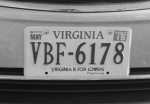
\includegraphics{figures/imtestes.png}
	\caption{Imagem de alta resolução utilizada nos testes.}
	\label{fig:hrimage}

\end{figure}

Para os testes feitos neste trabalho, a imagem de alta resolução foi reamostrada de forma que as dimensões das imagens de baixa resolução são iguais a $0.25$ vezes as dimensões da imagem HR.  
Dessa forma, há 16 pontos na imagem de alta resolução para cada ponto na imagem de baix resolução.
A largura da função de espalhamento de ponto ($\gamma$) escolhida foi 2.
Para cada imagem, o ângulo de rotação foi escolhido aleatoriamente de uma distribuição uniforme entre $-4$ e $4$ graus.
A mesma seleção aleatória foi feita para o deslocamento linear da imagem; a quantidade de pontos de deslocamento foi retirada de uma distribuição uniforme e contínua entre $-2$ e $2$ em cada um dos eixos.
A tabela \ref{tab:resumoParametros} resume os parâmetros utilizados na degradação das imagens.

\begin{figure}[H]
	\centering
	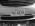
\includegraphics{figures/degradedImg/result-0.png}
	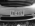
\includegraphics{figures/degradedImg/result-1.png}
	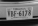
\includegraphics{figures/degradedImg/result-2.png}
	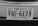
\includegraphics{figures/degradedImg/result-3.png}
	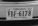
\includegraphics{figures/degradedImg/result-4.png}
	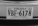
\includegraphics{figures/degradedImg/result-5.png}
	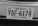
\includegraphics{figures/degradedImg/result-6.png}
	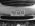
\includegraphics{figures/degradedImg/result-7.png}
	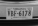
\includegraphics{figures/degradedImg/result-8.png}
	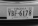
\includegraphics{figures/degradedImg/result-9.png} \\
	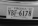
\includegraphics{figures/degradedImg/result-10.png}
	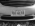
\includegraphics{figures/degradedImg/result-11.png}
	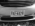
\includegraphics{figures/degradedImg/result-12.png}
	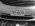
\includegraphics{figures/degradedImg/result-13.png}
	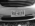
\includegraphics{figures/degradedImg/result-14.png}
	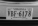
\includegraphics{figures/degradedImg/result-15.png}
	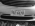
\includegraphics{figures/degradedImg/result-16.png}
	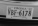
\includegraphics{figures/degradedImg/result-17.png}
	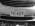
\includegraphics{figures/degradedImg/result-18.png}
	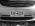
\includegraphics{figures/degradedImg/result-19.png}
	\caption{Conjunto das imagens geradas a partir da imagem de alta resolução. A diferença sutil entre as imagens é causada pelas transformações de deslocamento e rotação.}
	\label{fig:frames}
\end{figure}

\begin{table}[h]
	\centering
	\caption{Parâmetros de degradação usados para gerar o conjunto de imagens de teste.}
	\label{tab:resumoParametros}
	\begin{tabular}{r | l}
		Ângulos de rotação ($\theta_k$) & $ \sim \mathcal{U}(-4, 4)$ \\ \hline
		Deslocamento ($\mathbf{s}_k$)& $\sim \mathcal{U}(-2,2)$\\ \hline
		Largura da PSF ($\gamma$) & 2 \\ \hline
		Dimensões da imagem de alta resolução & $139 \times 104$ \\ \hline
		Dimensões das imagens de baixa resolução & $35 \times 26$ \\

	\end{tabular}
\end{table}

O processo de geração das imagens de baixa resolução foi todo desenvolvido usando a linguagem Python,
beneficiando-se dos módulos Numpy e Pillow.
Os parâmetros de degradação bem como as dimensões da imagem original foram salvas em arquivos de valores separados por vírgula (csv) junto com as imagens geradas.
Isso foi necessário para que fosse possível validar os resultados das etapas de restauração.

\section{Estimação dos parâmetros de degradação}
\label{sec:parestimation}
A primeira etapa no processo de restauração da imagem é estimar os parâmetros que definiram as transformações que degradaram a imagem durante o processo simulado de captura.Como já elucidado no capítulo \ref{chap:srbayes}, encontrar os valores dos parâmetros de degradação é um problema de otimização.
Teoricamente, os valores verdadeiros de $\mathbf{s}_k$, $\theta_k$ e $\gamma$ são os que maximizam a função de verosimilhança em \ref{eq:parameter}.

O artigo no qual este trabalho se baseia relata que o método de otimização usado para estimar tanto os parâmetros de degradação quanto a imagem foi o de gradientes conjugados \cite{tipping2003bayesian}.
Este algorítimo de otimização também é usado neste trabalho, porém com algumas diferenças na implementação.

Como a função em \ref{eq:parameter} não é uma função vetorial do tipo $ f(\mathbf{x}) : \mathbb{R}^n \to \mathbb{R}^1 $.
Por isso, a função de verossimilhança foi empacotada de forma que receba todos os parâmetros de entrada na forma de um vetor e retorne somente um escalar na saída.

Ambos os procedimentos de geração das imagens de teste e otimização foram desenvolvidos na linguagem Python, usando seus módulos Numpy, Scipy e Pillow.

Em vez de otimizar todos os parâmetros ao mesmo tempo,
constatou-se que a otimização converge mais rápido se os valores 

\section{Estimação da imagem de alta resolução}
